\documentclass[UTF8]{ctexart}
\usepackage{graphicx} % Required for inserting images

\title{测量碘钟反应颜色变化}
\author{BrightMoon}
\date{June 2024}

\begin{document}

\maketitle

\section{实验步骤}
\begin{enumerate}
    \item 将之前插在面包板上的电路,转移焊接在电路板上。结果如图\ref{实验电路}。
    \item 编写LavVIEW代码,测量电路输出信号,见图\ref{LabVIEW代码}。
    \item 取比色皿,首先加入碘钟反应的B液、C液各700$\mu L$。
    \item 为了减小环境光源不稳定带来的干扰,将比色皿尽量贴近光电二极管放置。
    \item 准备好测量装置后,加入A液700$\mu L$, 开始碘钟反应,同时开始测量。
\end{enumerate}

\begin{figure}
    \centering
    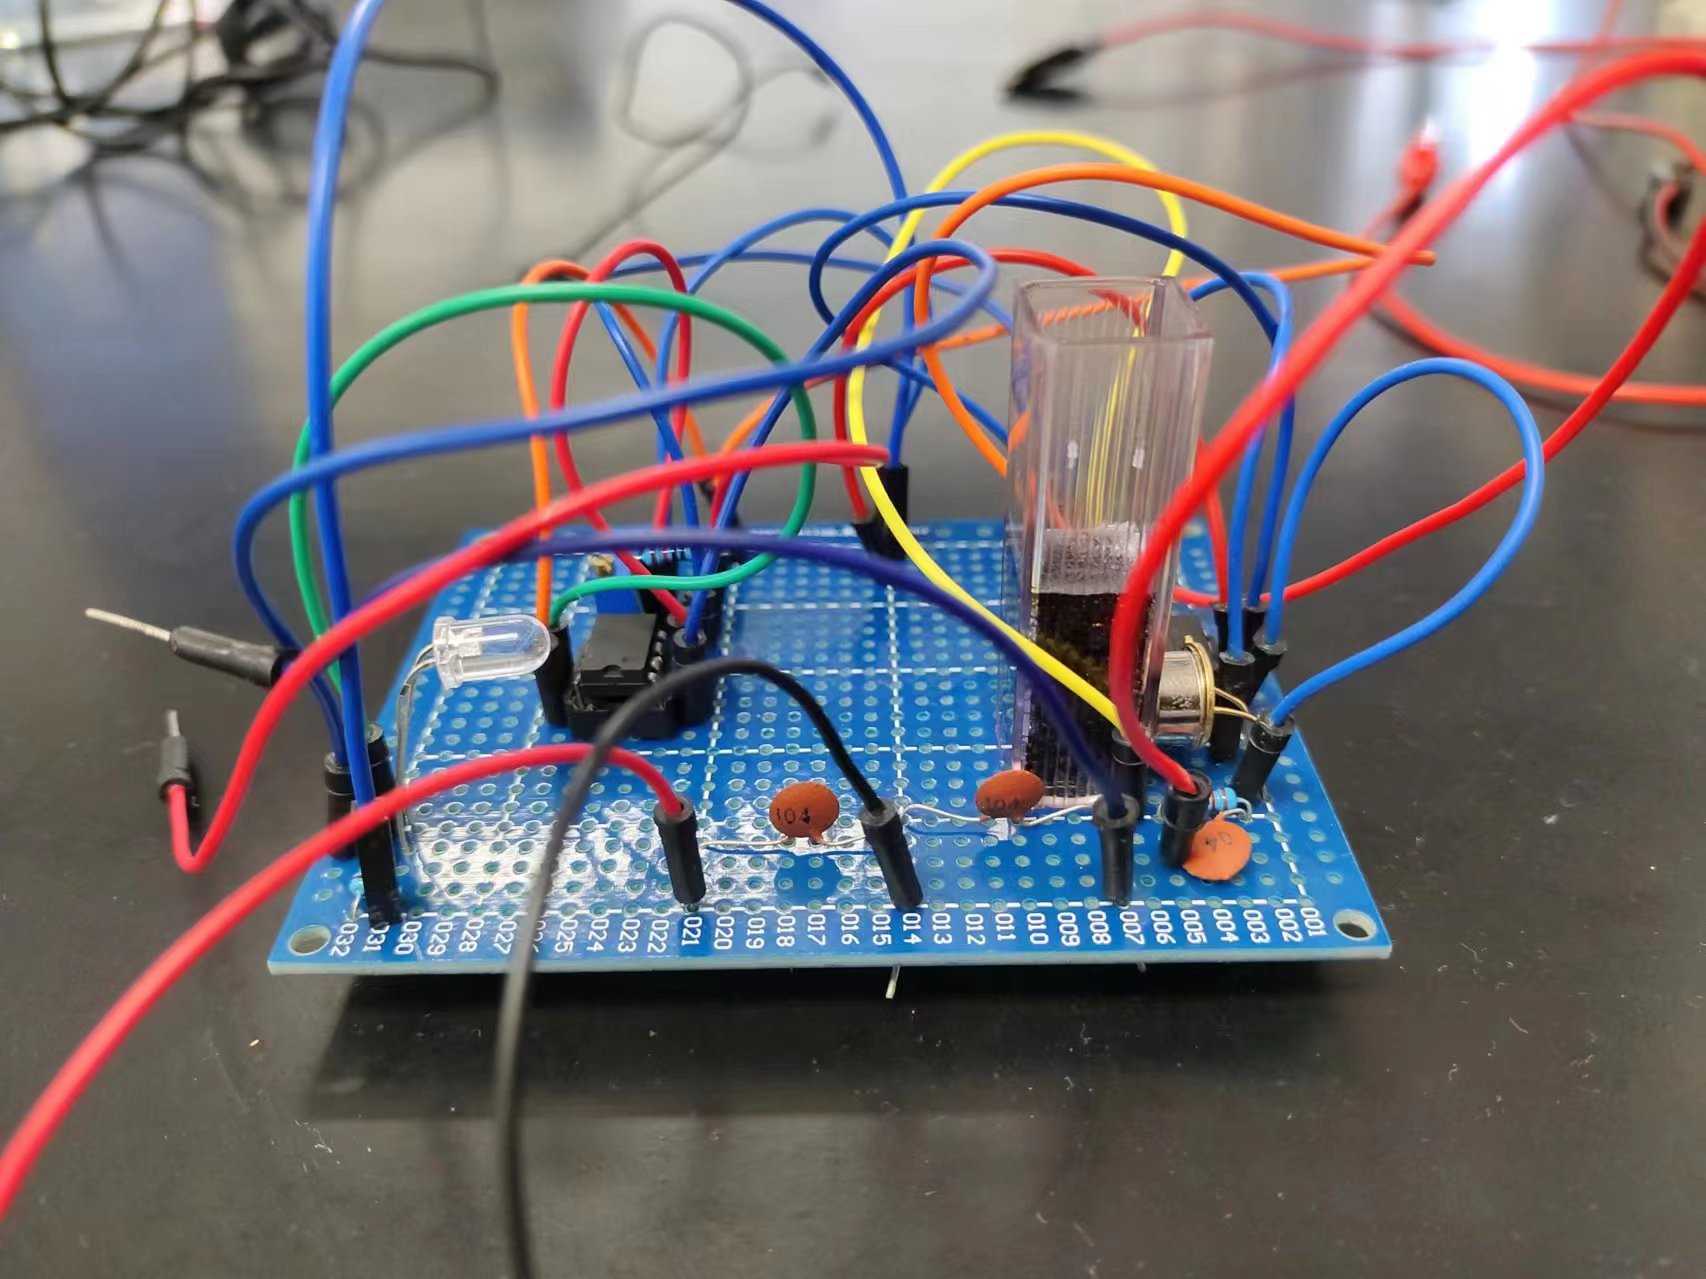
\includegraphics[width=0.5\linewidth]{实验电路.jpg}
    \caption{实验电路}
    \label{实验电路}
\end{figure}
\begin{figure}
    \centering
    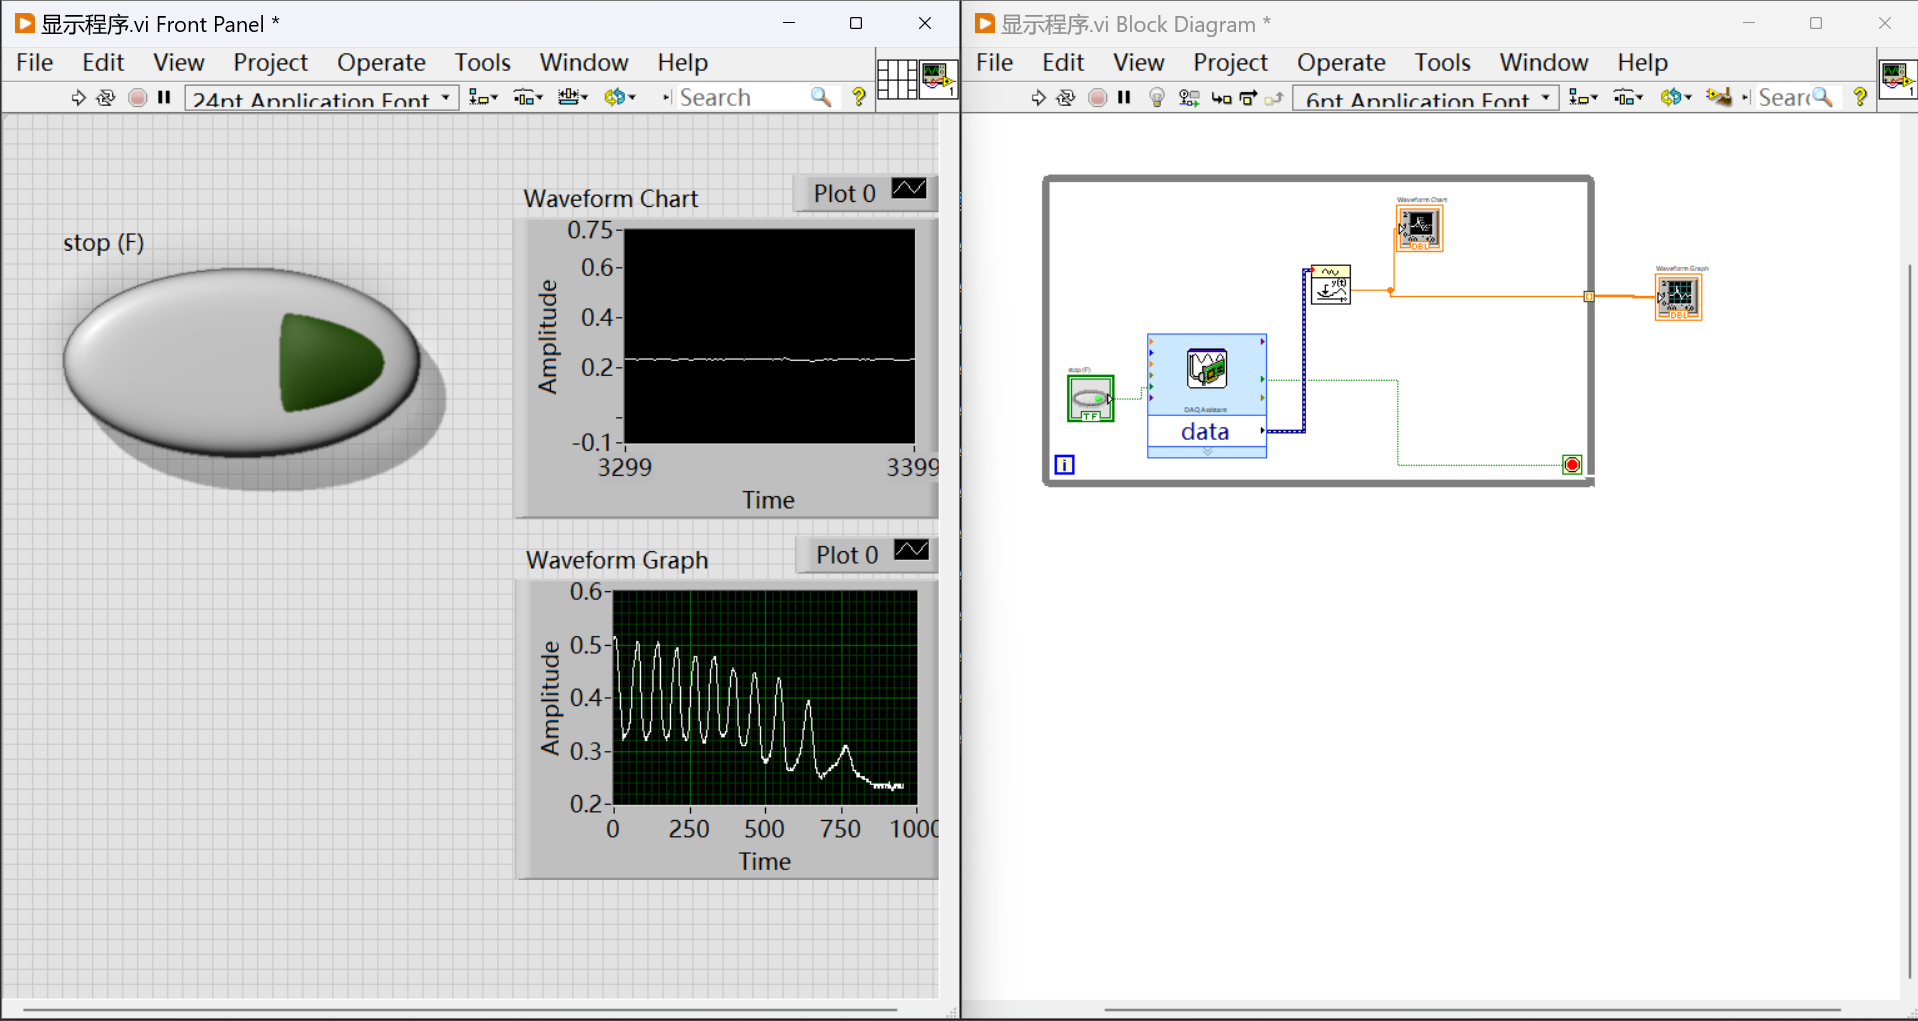
\includegraphics[width=0.75\linewidth]{检测结果显示程序.png}
    \caption{LabVIEW代码}
    \label{LabVIEW代码}
\end{figure}
\section{测量结果}
碘钟反应在一段时间内,颜色在深紫色和透明色之间周期性转变。
\begin{figure}
    \centering
    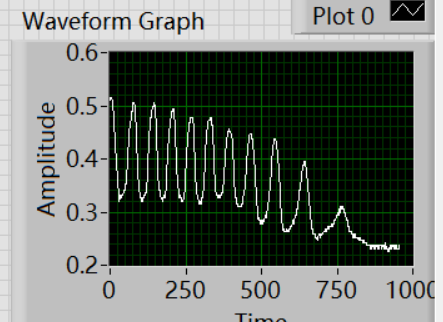
\includegraphics[width=0.75\linewidth]{检测结果1.png}
    \caption{测量结果}
    \label{测量结果}

\end{figure}
\begin{figure}
    \centering
    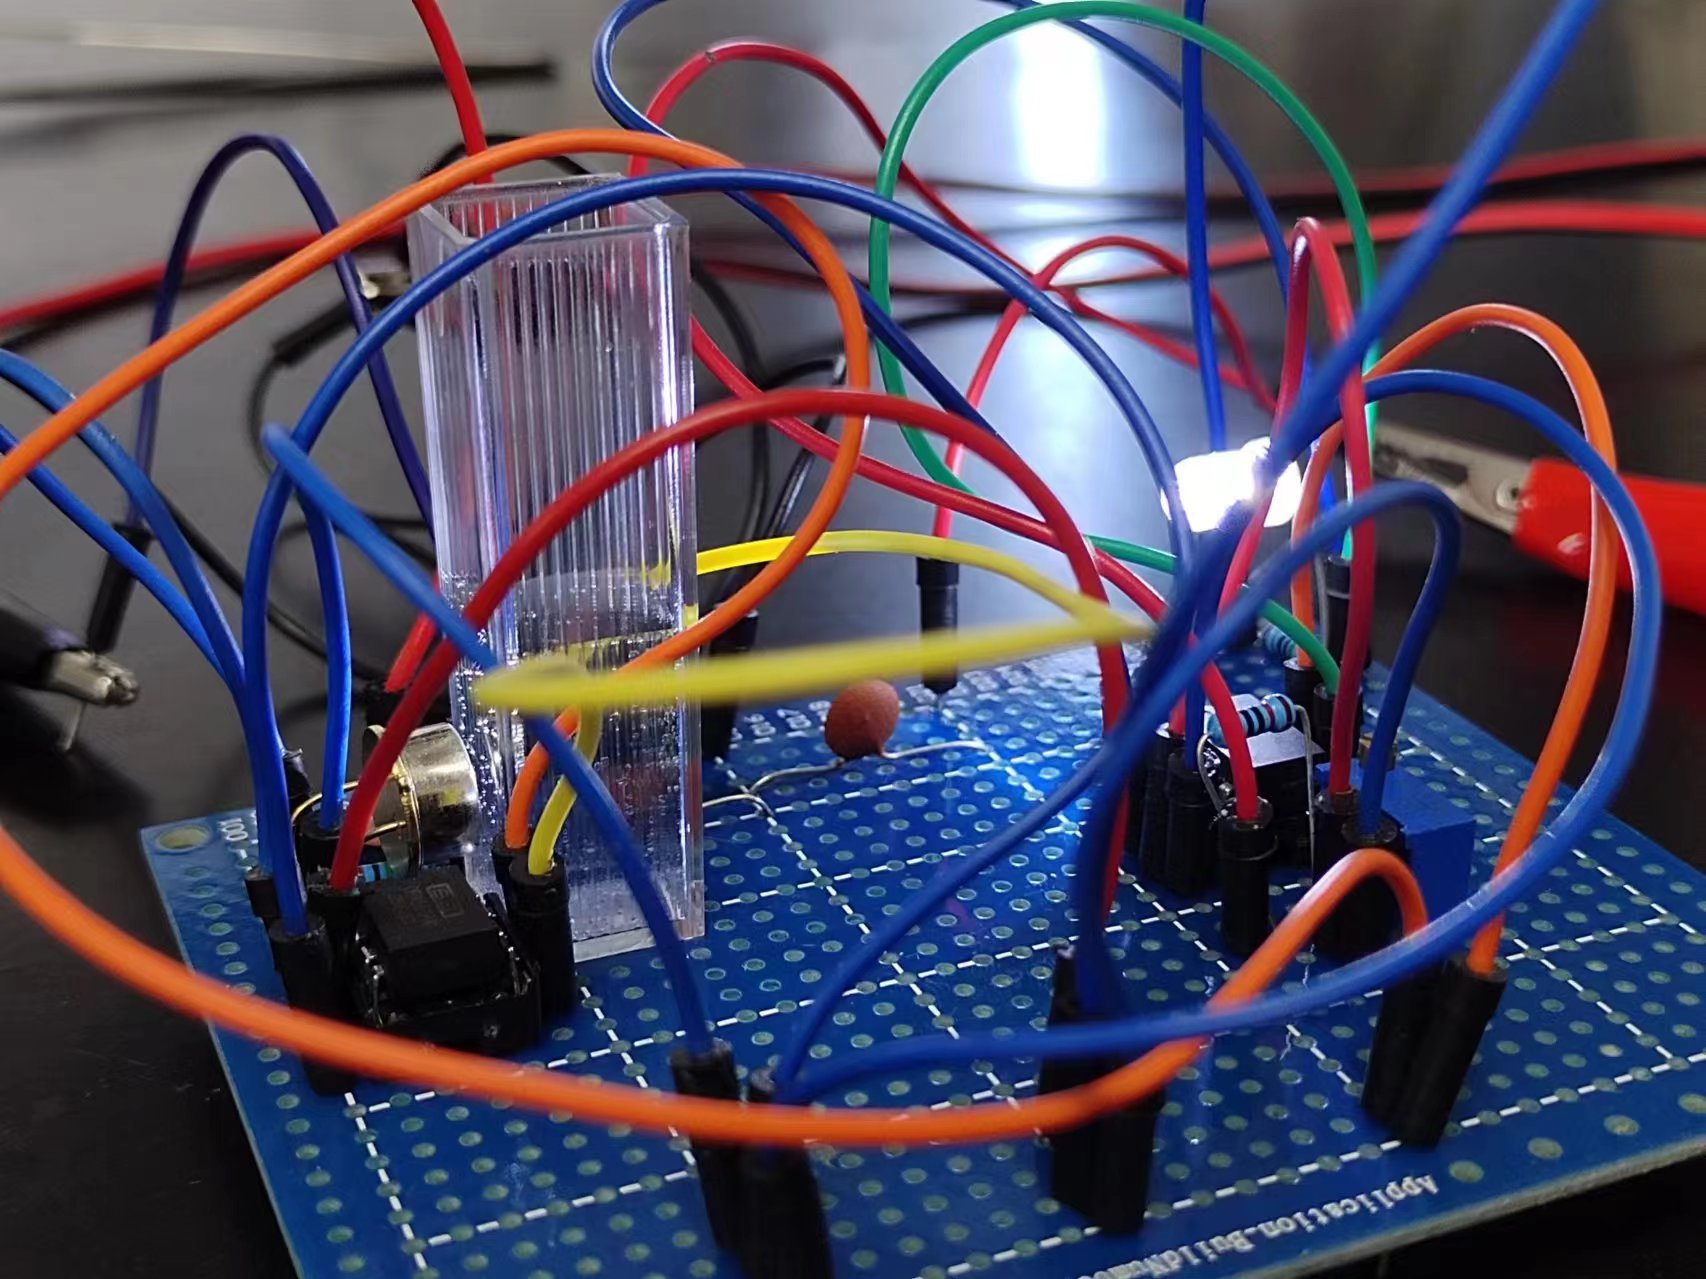
\includegraphics[width=0.75\linewidth]{测量过程.jpg}
    \caption{测量过程}
    \label{测量过程}
\end{figure}
\begin{enumerate}
    \item 从测量结果可以看出,透光率在周期性振荡中整体下降。
    \item 振荡的幅度逐步减小,并且最终趋向于零。与此同时,透光率降到最低,颜色稳定保持在深紫色。
\end{enumerate}
\end{document}
